\fancyhead[R]{\slshape PHỤ LỤC}
\begin{center}
	\begin{huge}
			\textbf{PHỤ LỤC 2}\\
			\textit{Công cụ Ollydbg}
	\end{huge}
\end{center}

\subsection*{Giới thiệu}
	OllyDbg là một công cụ sử dụng hợp ngữ trên nền Windows 32-bit chú trọng đến việc phân tích mã nhị phân. Công cụ dò xét các thanh ghi, nhận diện các thao tác với câu lệnh assmebly, các lời gọi hàm API, hằng số, chuỗi, từ khóa chuyển câu lệnh, cũng như chỉ ra địa chỉ thao tác từ tập tin và các thư viện. Công cụ ollydbg hoàn toàn miễn phí và đầy đủ chức năng, không có giới hạn thời gian sử dụng, nhưng có thông tin đăng ký với tác giả như ở các dạng phần mềm dùng thử. Các phiên bản hiện tại của OllyDbg không thể thao tác được các tập tin biên dịch cho các bộ vi xử lý 64-bit.
\subsection*{Thao tác}
Hình~\ref{fig:GiaoDienOllydbg} thể hiện giao diện chính của Ollydbg
	\begin{center}
			\begin{figure}[htp]
				\begin{center}
					\includegraphics[scale=0.75]{GiaoDienollydbg.png}
				\end{center}
				\caption{Giao diện công cụ Ollydbg}	
					\label{fig:GiaoDienOllydbg}		
			\end{figure}
		\end{center}		

File đầu vào của công cụ Ollydbg là một file thực thi có đuôi file là \textit{".exe"}. Để mở file, theo đường dẫn File->Open để chon nơi lưu file sau đó Click Open. Ngoài ra có thể thao tác click vào biểu tượng thư mục như hinh ~\ref{fig:OpenOllydbg} để mở file.
		\begin{center}
			\begin{figure}[htp]
				\begin{center}
					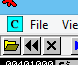
\includegraphics[scale=1]{OpenOllybdg.png}
				\end{center}
				\caption{Mở file trong Ollydbg}	
					\label{fig:OpenOllydbg}		
			\end{figure}
		\end{center}		
Khi mở một flie thực thi sẽ có giao diện như hình ~\ref{fig:VDOllydbg}
	\begin{center}
			\begin{figure}[htp]
				\begin{center}
					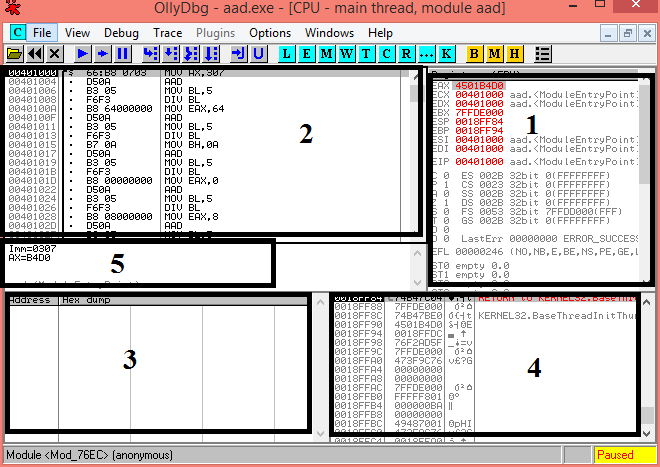
\includegraphics[scale=0.75]{VDOllydbg.png}
				\end{center}
				\caption{Ví dụ Ollydbg}	
					\label{fig:VDOllydbg}		
			\end{figure}
		\end{center}		
		
Giao diện khi mở một file thực thi có 5 cửa xổ
	
	\begin{itemize}
		\item[1] Cửa số thanh ghi (Registers): đây là cửa số chứa thông tin chi tiết về các thanh ghi như eax, ebx, ecx v….v…..Các cờ trạng thái cũng được quản lý tại cửa sổ này.
		\item[2] Cửa số giả mã assembly (Disassembler): cửa sổ này cho thấy các đoạn code của chương trình ở dạng ngôn ngữ assembly, và đồng thời tại cửa sổ này các bạn cũng có thể chú thích cho từng từng dòng mã assembly .
		\item[3] Cửa số giải mã giá trị (Dump): cửa sổ cho thấy bộ nhớ hiện tại của chương trình theo 2 dạng là hex và Ascii đồng thời cho phép chỉnh sửa bộ nhớ.
		\item[4] Cửa số stack:  mọi câu lệnh trước khi được thực hiện phải được nạp vào Stack.
		\item[5] Cửa số thông báo toán hạng (Tip):  Khi bạn đang ở tại một dòng code nào đó trong quá trình debug ,  Olly sẽ cho bạn thấy thông tin chi tiết về dòng code đó. Ví dụ  : nếu đang debug ở dòng lệnh \textit{ “ mov eax , dword ptr [123]”} . Thì cửa sổ này sẽ cho biết được giá trị hay con số nào đang được lưu giữ tại [123].
		\end{itemize}
	
	\subsubsection*{Cửa số Register}	
	Hình ~\ref{fig:OllydbgReg} thể hiện cửa số Register chứa các biến môi trường được dùng để thao tác với  mỗi câu lệnh.
	\begin{center}
			\begin{figure}[htp]
				\begin{center}
					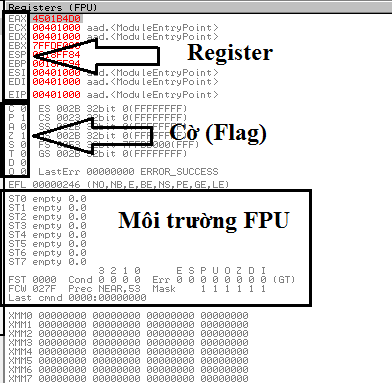
\includegraphics[scale=0.75]{OllydbgReg.png}
				\end{center}
				\caption{Cửa sổ Register trong Ollydbg}	
					\label{fig:OllydbgReg}		
			\end{figure}
		\end{center}		
		
		Cửa số này sẽ cung cấp rất nhiều thông tin trong quá trình chúng ta làm việc với Ollydbg. Các biến EAX, EBX, ECX, EDX, ... thể hiện các thanh ghi xử lý số nguyên. Các biến cờ C, P, A, Z... thay đổi trong quá trình thao tác với các câu lệnh số nguyên. Các biến ST0, ST1, ST2, ... FCW, FSW biểu diễn stack thanh ghi dữ liệu FPU, thanh ghi điều khiển FPU, thanh ghi trạng thái FPU.
		
	\subsubsection*{Cửa số Disassembler}
	Hình ~\ref{fig:OllydbgDisasm} thể hiện cửa sổ Disassembler, biểu diễn các câu lệnh assembly của chương trình đầu vào.. 
		\begin{center}
			\begin{figure}[htp]
				\begin{center}
					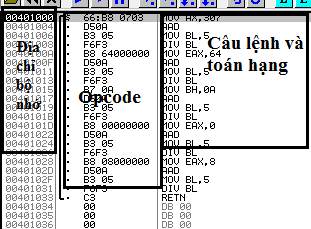
\includegraphics[scale=1]{OllydbgDisasm.png}
				\end{center}
				\caption{Cửa sổ Disassembler trong Ollydbg}	
					\label{fig:OllydbgDisasm}		
			\end{figure}
		\end{center}		
		
		Khi muốn debug một chương trình, cần phải load file thực thi của chương trình đó vào trong Ollydbg. Các chương trình mà đã được load vào Ollydbg là những chương trình có thể được code bằng những ngôn ngữ khác nhau như : VB, VC++, Borland Delphi hay MASM nhưng tại cửa sổ này toàn bộ code của chương trình sẽ được list ra dưới dạng các mã ASM. Ollydbg tiến hành phân tích chương trình và thể hiện chương trình dưới dạng assembly ở cửa số này đồng thời cung cấp tên câu lệnh assembly cùng với các toán hạng. Cho biết địa chỉ câu lệnh đang ở đâu trong bộ nhớ cùng mã opcode của câu lệnh assembly đang hiện hành. 
	
		\newpage
		\subsubsection*{Cửa sổ stack}
		Trước tiên sẽ đi tìm hiểu sơ qua về Stack. Đây là nơi lưu trữ tạm thời các dữ liệu và địa chỉ, nó là một cấu trúc dữ liệu một chiều. Các phần tử được cất vào và lấy ra từ một đầu của cấu trúc này, tức là nó được xử lý theo phương thức “vào trước, ra sau” (LIFO : Last In First Out). Phần tử được cất vào cuối cùng gọi là đỉnh của Stack. Có thể hình dung Stack như là một chồng đĩa, chiếc đĩa được đặt lên cuối cùng sẽ nằm trên đỉnh và chỉ có nó mới có thể được lấy ra đầu tiên. Hai thanh ghi chính làm việc với Stack là ESP và EBP. Theo mặc định trong Olly, Stack được biểu diễn theo thanh ghi ESP tuy nhiên ta có thể luân chuyển qua lại giữa ESP và EBP bằng cách nhấn chuột phải và chọn như hình~\ref{fig:OllydbgStack}
		\begin{center}
			\begin{figure}[htp]
				\begin{center}
					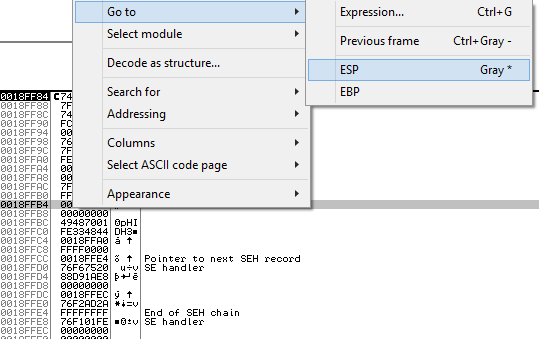
\includegraphics[scale=1]{OllydbgStack.png}
				\end{center}
				\caption{Cửa sổ Stack trong Ollydbg}	
					\label{fig:OllydbgStack}		
			\end{figure}
		\end{center}				
	
	\newpage	
	\subsubsection*{Cửa sổ Dump}
	Đây là cửa số hiện thị nội dung của bộ nhớ hoặc file. Ta có thể chọn nhiều định dạng khác nhau để biểu diễn nội dung của memory trong cửa số này : byte, text, integer, float, address, disassembly hoặc PE Header. Cửa sổ này cho phép chúng ta tìm kiếm cũng như  thực hiện các chức năng chỉnh sửa, thiết lập các Break points v..v... được thể hiện trong hình ~\ref{fig:OllydbgDump}.
	\begin{center}
			\begin{figure}[htp]
				\begin{center}
					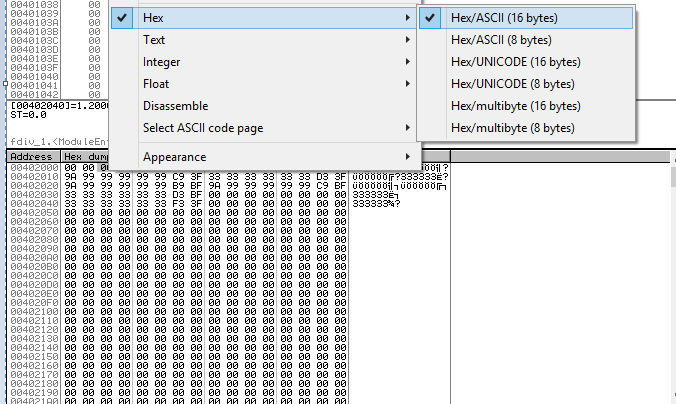
\includegraphics[scale=1]{OllydbgDump.png}
				\end{center}
				\caption{Cửa sổ Dump trong Ollydbg}	
					\label{fig:OllydbgDump}		
			\end{figure}
		\end{center}		
	
	\newpage
	\subsubsection*{Chức năng}
	Tiếp theo sẽ giới thiệu qua chức của từng nút trên thanh công cụ Ollydbg(hình ~\ref{fig:OllydbgBut} )
		\begin{center}
			\begin{figure}[htp]
				\begin{center}
					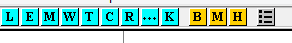
\includegraphics[scale=1]{OllydbgBut.png}
				\end{center}
				\caption{Chức năng trong Ollydbg}	
					\label{fig:OllydbgBut}		
			\end{figure}
		\end{center}		
		
		\begin{itemize}
			\item[•] 	Nút L dùng để mở cửa sổ Log của Olly, cửa sổ thể hiện những thông tin mà Olly ghi lại. Theo mặc định thì cửa số này sẽ lưu các thông tin về các module, import library hoặc các Plugins được load cùng chương trình tại thời điểm đầu tiên khi ta load chương trình vào Olly. Bên cạnh đó cửa sổ này cũng ghi lại các thông tin về các Break points mà chúng ta đặt trong chương trình.
			\item[• ] Nút E dùng để mở cửa sổ Executables, cửa sổ này thể hiện danh sách những file có khả năng thực thi được chương trình sử dụng như file exe, dlls, ocxs , v..v.. 
			\item[•] Nút M dùng để mở cửa sổ Memory, cửa sổ này sẽ cho chúng ta thông tin về bộ nhớ đang được sử dụng bởi chương trình.
			\item[• ] 	Nút T dùng để mở cửa sổ Threads, cửa sổ này liệt kê các Threads của chương trình.
			\item[•]  	Nút W dùng để mở cửa sổ Windows.
			\item[• ] 	Nút H dùng để mở cửa sổ Handles.
			\item[• ]  Nút \/ để mở cửa sổ Patches, cửa sổ này sẽ cho chúng ta các thông tin về những thông tin đã edit trong chương trình.
			\item[•]  Nút K để mở cửa sổ Call Stack, hiển thị một danh sách các lệnh call mà chương trình  đã thực hiện khi  Run bằng F9 và dùng F12 để tạm dừng chương trình.
			\item[•]  Nút B để mở cửa sổ Break Points, cửa sổ này sẽ hiển thị tất cả các BPs mà đã đặt trong chương trình. Tuy nhiên nó chỉ hiện thị các BPs được set bằng cách nhấn F2, còn các dạng BPs khác như : hardware breakpoint hoặc memory breakpoints thì không được liệt kê ra ở phụ lục này.
			\item[•] Nút R để mở cửa sổ References, cửa sổ này là kết quả khi hực hiện chức năng Search trong Ollydbg.	
		\end{itemize}		
	
	\subsubsection*{Phím tắt}
	\textbf{F7 : } Khi nhấn F7 sẽ thực thi từng dòng lệnh 1. Nếu trong quá trình thực thi mà gặp lệnh Call thì sẽ đi vào trong lòng của lệnh Call đó và thực thi từng câu lệnh trong lệnh Call này cho đến khi gặp lệnh Retn để trở lại chương trình chính, tức là câu lệnh tiếp theo sau lệnh Call.\\
	
		\textbf{F8 :} Cũng tương tự như F7 nhưng có 1 điểm khác biệt trong quá trình thực thi từng câu lệnh, nếu như gặp lệnh Call nó bỏ qua không cần quan tâm các lệnh bên trong lệnh Call mà thực thi luôn lệnh Call đó và dừng lại tại câu lệnh tiếp theo dưới lệnh Call.\\
		
		\textbf{F2 :} Đặt một Break point trong chương trình. Vậy Break point là gì , đơn giản nó chỉ là việc chúng ta tạo 1 điểm ngắt trong chương trình theo một điều kiện nào đó để khi thực thi chương trình, nếu thỏa điều kiện mà chúng ta đặt ra thì chương trình sẽ dừng lại tại vị trí mà chúng ta đã đặt BP.\\
		 
		\textbf{F9 :}  Cho phép thực thi chương trình trong chế độ Debug, tương tự như việc chúng ta nhấp đúp chuột vào chương trình để thực thi nó. Tuy nhiên khác với việc nhấp đúp chuột, nếu chúng ta nhấn F9 thì Olly sẽ tìm xem có BP nào được Set hay không, chương trình có hiện thị ra các Exception gì không, hay nếu chương trình có cơ chế chống Debug thì nó sẽ ngắt  ngay lập tức. Nếu như không có bất kì cản trở nào thì chương trình sẽ Run hoàn toàn và trên status bar của Olly sẽ báo cho chúng ta biết điều này.
		
		\textbf{F12 :} Tạm dừng chương trình lại.